\subsection{OpenMP}

The C++ OpenMP program is called through R via .Call() using the Rcpp interface. It accepts the same input arguments as the original function, can handle the same types of valid inputs, and through new optional arguments, also allows the user to decide on a scheduling policy and chunk size.\\
\null
Code highlights:\\
\begin{itemize}
\item Load balancing algorithm \cite{parallelalgorithm} (next section)
\item Avoidance of critical sections and barriers
\end{itemize}
Other notes:
\begin{itemize}
\item Similar to the original function, the OpenMP implementation has a limit on the input/output size. The program terminates if R decides that it cannot allocate enough space for the output.
\end{itemize}

\subsubsection{Load Balancing}
Good load balancing is very critical to our program because for each element $i$ in the input vector $x$, the number of combinations that can be generated with $x_{i}$ is larger than that with $x_{i+1}$. A naive task distribution without proper load balancing could heavily skew the distribution of the workload for each thread. For example, directly assigning an $x_{i}$ for each thread will result in the threads with lower id's generating far more combinations (thus, more work) than threads with higher id's).\\
\null
In order to compensate for the load imbalance, the assignment of tasks to the threads was done in a wrap around manner. Using this method, for the first distribution, each thread will work on the element indexed in the same value as their id (e.g. thread 0 on $x[0]$, thread 1 on $x[1]$, and so on). Then, the following distribution depends on the total number of threads, the id of each thread, and the index of its previous assignment. With $nth$ corresponding to the total number of threads and $me$ corresponding to the thread id, the assignment following the initial distribution is determined using the equation:
\begin{equation}
next\_task = prev\_task + 2 * (nth - me - 1) + 1
\end{equation}
The distribution that will then follow the above depends on the id of each thread the index of the previous task. This next distribution is determined by the equation:
\begin{equation}
next\_task = prev\_task + 2 * me + 1
\end{equation}
The succeeding distributions alternates in using the two equations until the last distribution, which is for $n - m + 1$ or the last $x_{i}$ that can form a combination of size $m$ with the elements succeeding it.\\
\null
In this algorithm, each thread knows which indexes in $x$ to generate combinations for. The threads do not need to communicate with each other, avoiding huge overhead especially for large values of n.

\subsubsection{Chunk Size}
The equations from the section above implicitly defines the chunk size so that each thread gets assigned roughly the same number $x_{i}$'s to work on. It is essentially the number of times task distributions occur in the load balance algorithm, which is roughly $(n-m+1)/nth$.

\subsubsection{Scheduling Policies}
The load balancing algorithm described in Section 3.1.1 implements a static scheduling policy since the threads are assigned specific tasks and only work on the tasks assigned to them. For the purposes of timing comparisons, additional optional arguments \texttt{sched} and \texttt{chunksize} were added to the function in order to test the speed of the program for the other scheduling policies, namely dynamic and guided. If both arguments are not provided (or set as NULL), the program defaults to the static scheduling policy using the load balancing algorithm. If either dynamic or guided is set, the program uses OpenMP's built-in \texttt{schedule} clause to distribute the tasks to the threads. If the chunksize is not provided, the program sets it to the default chunk size of 1.\\
\null

We performed various tests using the three scheduling policies and experimented with different chunk sizes (for dynamic and guided). It was clear that the load balancing algorithm using static scheduling was the fastest. It eliminates the communication overhead of the dynamic and guided scheduling policies since the threads don't have to repeatedly access the task farm for work, and idleness is still reduced because of the way the tasks are distributed among the threads.\\
\null

Hence, the static method is the one compared to the original function in the timinng comparisons.

\subsubsection{Cache and Other Performance Tuning Considerations}
The following performance tuning applies only to the load balancing algorithm described in 3.1.1.

\begin{itemize}
\item Avoiding instances of false sharing: In order to avoid instances of false sharing (and the resulting cache coherence overheads), we avoided having shared data that could be modified by multiple threads. The data frequently accessed and shared by the threads in the program, such as the input and position vectors are read-only data. Hence, cache lines are not invalidated whenever data from these vectors are accessed. The main shared data structure that is modified by all threads is the output matrix \texttt{retmat}, but the threads never have to perform any read on this data.

\item Synchronization overhead: The threads are made to work as independent of each other as possible. The only synchronization occurs implicitly at the end of the \texttt{parallel} pragma.

\item Avoidance of critical sections and barriers

\end{itemize}


\subsubsection{Comparative Analysis}
The following input sizes were used for comparing the speeds of the source code and our OpenMP implementation using 8 threads. Tests were done using \texttt{system.time(combn(sample(1:n), m))}.\\
\null

\texttt{> nCm(100, 2, 0.10000000000000002)}\\
\texttt{[1] 4950}\\
\texttt{> nCm(300, 2, 0.10000000000000002)}\\
\texttt{[1] 44850}\\
\texttt{> nCm(100, 3, 0.10000000000000002)}\\
\texttt{[1] 161700}\\
\texttt{> nCm(150, 3, 0.10000000000000002)}\\
\texttt{[1] 551300}\\
\texttt{> nCm(200, 3, 0.10000000000000002)}\\
\texttt{[1] 1313400}\\
\texttt{> nCm(250, 3, 0.10000000000000002)}\\
\texttt{[1] 2573000}\\
\texttt{> nCm(300, 3, 0.10000000000000002)}\\
\texttt{[1] 4455100}\\
\null

The elapsed time recorded for each test is the average of three trials. The OpenMP parallelization massively improved the performance of the function. The improvement becomes increasingly invaluable as the input size increases (e.g. \texttt{nCm(100, 5)}, the OpenMP implementation still manages to produce an output under 5 seconds, while the original function takes several minutes).\\
\null

The following plot illustrates the differences in the speeds of the two implementations.\\
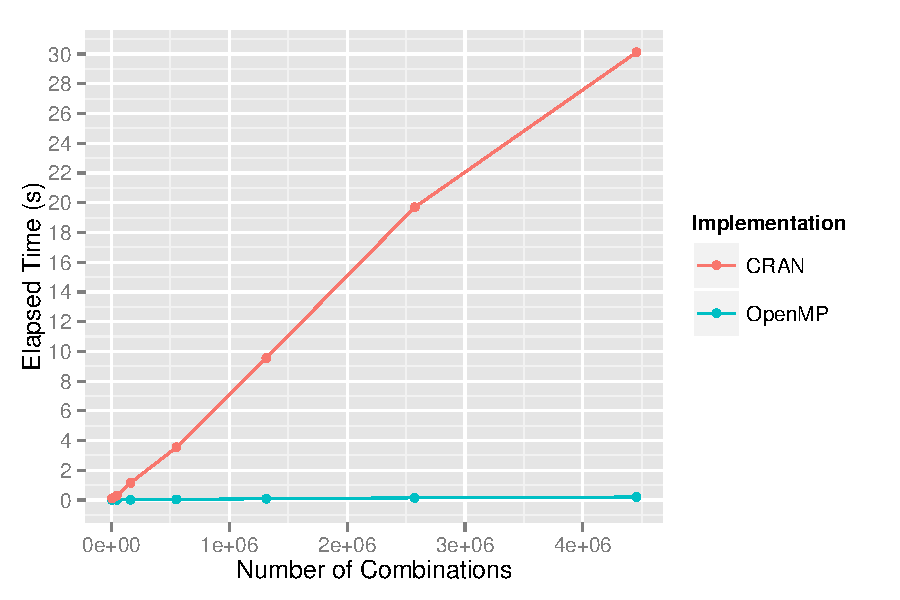
\includegraphics{openmp.pdf}

